\documentclass[a4paper]{article}

\usepackage{giacomo}

\usepackage{wrapfig}
\usepackage{float}

\begin{document}
\author{Giacomo Borin}
\title{Geometria B definizioni}
\maketitle

\section{Teoria degli Insiemi}
Consideriamo due insiemi $X$ e $Y$ e una funzione $ f:X \to Y$, sia poi $A$ un sottoinsieme di $X$, $ \{ A_i \} _{i \in I } \subset X $ una famiglia di sottoinsiemi di $X$ \footnote{In realtà questo sarebbe un abuso di notazione, utilizzato per indicare una applicazione da un insieme $I$ non vuoto (detto insieme degli indici) nelle parti di $X$: $\phi: I \to X$, dove abbiamo indicato $\phi(i)$ con $A_i$ per ogni $i$ in $I$}, mentre $B$ un sottoinsieme di $Y$ e  $\{ B_i \} _{j \in J } \subset Y $ una famiglia di sottoinsiemi di $Y$. L'isieme dei sottoinsiemi di $X$ si dice insieme delle parti di $X$ e si indica con $\Parts (X)$. Mentre l'insieme complementare di $A$ in $X$ è l'insieme degli elementi di $X$ non contenuti in $A$, e si indica con $\comp{X}(A)$ \\
Valgono allora i seguenti fatti: 
\begin{itemize}
	\item $ f^{-1} ( f(A)) \supset A $ 
	\item $f$ iniettiva $\Leftrightarrow f^{-1} ( f(A)) = A $ 
	\item $f(f^{-1} ( B)) = B \cap f(X) $ 
	\item $f$ è suriettiva $\Leftrightarrow f(f^{-1} ( B)) = B $.
	\item $ \comp{X} ( \bigcup_{i \in I} A_i ) = \bigcap _{i \in I} \comp{X} (A_i) $ \footnote{Questa formula e quella successiva sono dette formule di De Morgan}
	\item $ \comp{X} ( \bigcap_{i \in I} A_i ) = \bigcup _{i \in I} \comp{X} (A_i) $ 
	\item $ f(\bigcup A_i ) = \bigcup _i  f(A) $
	\item $ f(\bigcap A_i ) \subset \bigcap _i  f(A) $ (in generale non vale l'uguaglianza)
	\item $ f^{-1} (\bigcup B_j ) = \bigcup f^{-1} (B_j ) $
	\item  $ f^{-1} (\bigcap B_j ) = \bigcap f^{-1} (B_j ) $ 
	\item $ \comp{X} (f^{-1} (B)) = f \inv (\comp{Y} (B)) $
\end{itemize}

\section{Topologia}
D'ora in poi X è sempre un insieme non vuoto dato che non siamo interessati a fare una trattazione dei casi banali.
\begin{deff} 
Una topologia su X è una famiglia $\tau \subset \Parts ( X) $ che soddisfa le seguenti tre propietà: 
\begin{enumerate} 
\item $\{ \phi , X \} \in \tau $ 
\item $\tau $ stabile per unione arbitraria 
\item $\tau $ stabile per unione finita
\end{enumerate}
\end{deff}
\begin{oss} La terza condizione può essere sostituita da: \\
se $ A_1 , A_2 \in \tau \Rightarrow A_1 \cap A_2 \in \tau $
\end{oss}

\begin{deff}
Su uno spazio metrico $(X,d ) $ è definita una topologia indotta dalla distanza $d$, indicata con $\tau _d $, che vede come aperti gli insiemi che sono unione di palle (dischi) della forma $B_d (x,r) =\{ y \in X | d(x,y) < r \} $ dove $ x \in X, r \in \R ^+ $. 
\end{deff}

\begin{deff}
Se uno spazio topologico $((X,\tau ) $ ammette una distanza \\ $ d : X \times X \to \R $ tale che $\tau = \tau _d $ allora lo spazio topologico si dice metrizzabile. 
\end{deff}
\begin{oss} Non tutti gli sapzi sono metrizzabili: ad esempio la topologia banale su uno spazio con $|X| \geq 2 $ non lo è.
\end{oss} 

\begin{deff}
Due topologie $ \tau $ e $ \tau '  $ su X si dicono confrontabili se $  \tau \supset ( \subset)  \tau '  $. Allora si dirà che $\tau $ è piu (meno) fine di $ \tau ' $ e si indicherà con $\tau \succeq (\preceq ) \tau ' $.
\end{deff}

\begin{oss}
l'intersezione arbitraria di topologie è ancora una topologia
\end{oss}

\section{Basi e sottobasi} 

\begin{deff}
Dato spazio topologico $(X,\tau )$, allora $\B \subset \tau $ si dice base se soddisfa una delle seguenti: 
\begin{enumerate}
\item Se ogni elemento della topologia è unione di elementi della base. Cioè 
	\begin{equation*}
	\tau = \{ A \in \Parts (X) | \exists \Lambda \subset \B . \bigcup _{B \in \Lambda } B = A \}
	\end{equation*}
\item Se $\forall A \in \tau . \forall x \in A . \exists B_x \in \B $ t.c. $ x \in B_x \subset A $.
\end{enumerate}
\end{deff}

\begin{prop}
Sia X un insieme non vuoto e sia $\B \subset \Parts (X) $, supponiamo che valgano:
	\begin{enumerate}
	\item $\B$ è ricoprimento di X
	\item $\forall B_1 , B_2 \in \B . \: B_1 \cap B_2 $ è unione di elementi di $ \B $ 
	\end{enumerate}
allora esiste un'unica topologia $\tau _{\B} $ che ha $ \B $ come base, ed è la meno fine contente $\B $, cioè è la topologia generata da $\B $.
\end{prop}

\begin{deff}
Sia $(X,\tau )$ spazio topologico e sia $\mathcal{S} \subset \tau $, allora $\mathcal{S}$ è sottobase di $\tau $ se la famiglia delle sue intersezioni \emph{finite} è una base di $ \tau $. \\
Oppure equivalentemente se $\forall A \in \tau \: : \, \forall x \in A. \, \exists \{U_i \}_{i=1} ^{n(x)} \subset \mathcal{S} $ t.c. $ x \in \bigcap_{i=1} ^n U_i \subset A $.
\end{deff}

\begin{prop}
Sia X un insieme non vuoto e sia $\mathcal{S} \subset \Parts (X) $, supponiamo che $\mathcal{S} $ sia un ricoprimento di X
allora esiste un'unica topologia $\tau _{\mathcal{S} } $ che ha $ \mathcal{S} $ come sottobase, inoltre $\tau _{\mathcal{S} } $ è la topologia generata da $\mathcal{S} $.
\end{prop}

\section{Intorni e basi di intorni} 

\begin{deff}[Intorno]
	
  

Dato spazio topologico $(X,\tau )$, $M \in \Parts (X) $, allora un sottoinsieme U di X si dice intorno di M in  $(X,\tau )$ se $\exists A \in \tau | M \subset A \subset U $.\\
Definiamo inoltre il \emph{sistema di intorni di x in $(X, \tau ) $} come: 
\begin{equation*} 
\mathcal{N} _{(\tau)} (x) = \{ U \in \Parts (X) | \exists A \in \tau . \: x \in A \subset U \} 
\end{equation*}


\tikzset{every picture/.style={line width=0.75pt}} %set default line width to 0.75pt        

\begin{center}
	
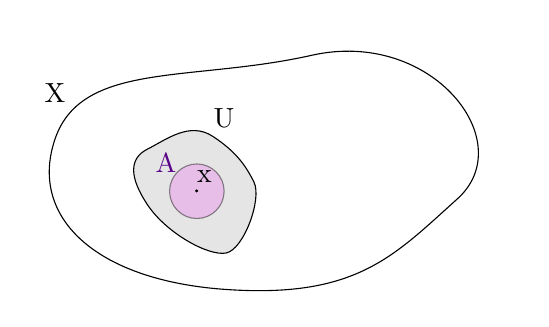
\begin{tikzpicture}[x=0.75pt,y=0.75pt,yscale=-1,xscale=1]
%uncomment if require: \path (0,300); %set diagram left start at 0, and has height of 300

%Shape: Polygon Curved [id:ds19507672643308271] 
\draw   (117.6,58.08) .. controls (130.63,20.78) and (183.21,31.12) .. (241.18,18.08) .. controls (299.15,5.05) and (341.85,59.88) .. (311.29,87.29) .. controls (280.73,114.71) and (262.75,135.38) .. (199.39,130.88) .. controls (136.02,126.39) and (104.56,95.38) .. (117.6,58.08) -- cycle ;
%Shape: Polygon Curved [id:ds4647277324799244] 
\draw  [fill={rgb, 255:red, 0; green, 0; blue, 0 }  ,fill opacity=0.1 ] (162.09,63.25) .. controls (171.07,58.76) and (182.31,49.77) .. (193.54,57.18) .. controls (204.78,64.6) and (209.31,71.18) .. (213.32,79.2) .. controls (217.33,87.23) and (208.37,111.78) .. (199.84,113.36) .. controls (191.3,114.93) and (171.07,103.7) .. (162.09,90.21) .. controls (153.1,76.73) and (153.1,67.74) .. (162.09,63.25) -- cycle ;
%Shape: Ellipse [id:dp3844106230202865] 
\draw  [color={rgb, 255:red, 0; green, 0; blue, 0 }  ,draw opacity=0.43 ][fill={rgb, 255:red, 233; green, 51; blue, 235 }  ,fill opacity=0.22 ] (172.65,83.58) .. controls (172.65,76.33) and (178.53,70.44) .. (185.79,70.44) .. controls (193.05,70.44) and (198.94,76.33) .. (198.94,83.58) .. controls (198.94,90.84) and (193.05,96.73) .. (185.79,96.73) .. controls (178.53,96.73) and (172.65,90.84) .. (172.65,83.58) -- cycle ;
%Flowchart: Summing Junction [id:dp7924193701587547] 
\draw  [fill={rgb, 255:red, 0; green, 0; blue, 0 }  ,fill opacity=1 ] (186.13,83.43) .. controls (186.13,83.65) and (185.95,83.83) .. (185.73,83.83) .. controls (185.5,83.83) and (185.32,83.65) .. (185.32,83.43) .. controls (185.32,83.2) and (185.5,83.02) .. (185.73,83.02) .. controls (185.95,83.02) and (186.13,83.2) .. (186.13,83.43) -- cycle ; \draw   (186.01,83.71) -- (185.44,83.14) ; \draw   (185.44,83.71) -- (186.01,83.14) ;

% Text Node
\draw (111.15,30.26) node [anchor=north west][inner sep=0.75pt]   [align=left] {X};
% Text Node
\draw (192.66,42.39) node [anchor=north west][inner sep=0.75pt]   [align=left] {U};
% Text Node
\draw (164.62,63.96) node [anchor=north west][inner sep=0.75pt]  [color={rgb, 255:red, 90; green, 5; blue, 137 }  ,opacity=1 ] [align=left] {A};
% Text Node
\draw (184.67,72.5) node [anchor=north west][inner sep=0.75pt]   [align=left] {x};


\end{tikzpicture}

\end{center}

\end{deff}



\begin{osss} \mbox{} \par
\begin{enumerate}
	\item se $U \in \mathcal{N} _{(\tau)} (x) $, allora $x \in U$
 	\item per ogni $ U \in \mathcal{N} _{(\tau)}  (x)$ esiste un $ A \in \tau $ tale che $x \in A \subset A \subset U$. Cioè a meno di restrizioni ogni intorno può essere considerato aperto (infatti basta considerare l'aperto della definizione).
 	\item se $U \in \mathcal{N} _{(\tau)}  (x)$ e $ V \in \Parts (X) $ t.c. $V \supset U \Rightarrow V \in \mathcal{N} _{(\tau )} (x)$ 
	\item $\mathcal{N} _{(\tau )} (x) $ stabile per intersezione finita.
	\item se $ U \in \mathcal{N} _{(\tau )} (x) $ allora $\exists V \in \mathcal{N} _{(\tau )} (x) $ t.c. $\forall y \in V \to V \in \mathcal{N} _{(\tau )} (y) $.
\end{enumerate}
\end{osss}

\begin{prop}
Sia $(X,\tau ) $ spazio topologico, allora A è aperto se e solo è intorno di ogni suo punto, o equivalentemente se e solo se $ A \in \bigcap _{x \in A } \mathcal{N} _{(\tau)} (x) $.
\end{prop}

\begin{prop}
Sia X insieme non vuoto, supponiamo di avere una funzione: 
\funmap{\mathcal{N}}{X}{\Parts (\Parts (X)) }{x}{ \mathcal{N} (x) }
tale che per ogni $ x \in X$ vale che:
\begin{enumerate}
	\item[0.] $ \mathcal{N} (x) \neq \phi $
	\item se $U \in \mathcal{N} (x) $, allora $x \in U$
	\item $\mathcal{N}  (x) $ stabile per intersezione finita.
 	\item se $U \in \mathcal{N}  (x)$ e $ V \in \Parts (X) $ t.c. $V \supset U \Rightarrow V \in \mathcal{N}  (x)$
	\item se $ U \in \mathcal{N} (x) $ allora $\exists V \in \mathcal{N}  (x) $ t.c. $\forall y \in V \to V \in \mathcal{N} (y) $.
\end{enumerate}
allora esiste un'unica topologia $\tau $ su X tale che $\forall x \in X . \,  \mathcal{N} (x) = \mathcal{N} _{\tau } (x) $, cioè vede $\mathcal{N} (x) $ come sistema di intorni di x.
\end{prop}

\begin{deff}
Sia $(X,\tau ) $ spazio topologico e sia $x \in X $, una famiglia $\mathcal{V} _{\tau } (x) $ di intorni di X si dice \emph{sistema fondamentale di intorni} di x in $(X,\tau )$ se per ogni $U \in \mathcal{N} _{\tau } (x)$ esiste $ V \in \mathcal{V} _{\tau } (x)$ t.c. $V \subset U $. Viene anche detto \emph{base di intorni} e viene abbreviato come S.F.I. di x.
\end{deff}

\begin{prop}
Sia $\mathcal{V} _{\tau } (x) $ un S.F.I. di x in $(X,\tau )$ allora A è aperto se solo se $\forall x \in A\, \exists V_x \in \mathcal{V} _{\tau } (x) $ t.c. $ V_x \subset A $.
\end{prop}

\begin{prop}
Sia $(X, \tau ) $ spazio topologico e $\B \subset \tau $, allora $\B $ è una base per $\tau $ se e solo se $\forall x \in X$ la famiglia $\B (x) = \{ B \in \B | B \ni x \} $ è un S.F.I. per x in $(X,\tau )$.
\end{prop}

\begin{cor}
Sia $(X, \tau ) $ spazio topologico e supponiamo di aver assegnato un S.F.I. per ogni x. Allora $ \B := \bigcup _{x \in X} \mathcal{V} (x) \subset \tau $ è una base di $\tau $. 
\end{cor}

\begin{prop}
Sia X un insieme non vuoto, supponiamo di avere una mappa
\funmap{\mathcal{V}}{X}{\Parts (\Parts (X))}{x}{\mathcal{V} (x) }
che per ogni $x \in X$ soddisfa le seguenti propietà:
	\begin{enumerate}
	\item[0.] $\mathcal{V}(x) \neq \phi $
	\item Se $V \in \mathcal{V}(x)$ allora $x \in V$
	\item Se $V_1 , V_2 \in \mathcal{V}(x) $ allora esiste $ V \in \mathcal{V}(x) | V \subset V_1 \cap V_2 $ 
	\item Sia $V \in \mathcal{V}(x) $ allora esiste $ A \in \Parts (X) | \, x \in A \subset V $ e $ \forall y \in A . \exists W_y \in \mathcal{V}(y) $ t.c. $ W_y \subset V $
	\end{enumerate}
allora esiste un'unica topologia $\tau $ che vede V come S.F.I.
\end{prop}

\section{Assiomi di numerabilità}

\begin{deff} Uno spazio topologico $(X, \tau ) $ soddisfa il \emph{primo assioma di numerabilità} se per ogni $x \in X$ ammette un S.F.I. di cardinalità numerabile
\end{deff}

\begin{oss} se uno spazio topologico soddisfa il primo assioma di numerabilità possiamo sempre trovare per ogni $x \in X$ un S.F.I. di x tale che $\mathcal{V}(x) = \{ V_n \}_{n \in \N } $ e $ V_n \supset V_{n+1} \, \forall n \in \N $
\end{oss}

\begin{deff} Uno spazio topologico $(X, \tau )$ soddisfa il \emph{secondo assioma di numerabilità} se $\tau $ ammette base numerabile 
\end{deff}

\begin{lem} se uno spazio topologico soddisfa il secondo assioma di numerabilità soddisfa anche il primo, ma non è vera l'implicazione inversa
\end{lem}

\begin{ex}[Spazio topologico che soddisfa il primo assioma ma non il secondo] Basta considerare un qualsiasi insieme X non numerabile e la topologia discreta, i come sistema di intorni per ogni x basta $\{ \{x \} \} $ (finito) però ogni base deve contenere almeno il singoletto per ogni punto, quindi non può essere numerabile.
\end{ex}

\begin{teo}(di Lindeloff) Dato uno spazio topologico $(X , \tau )$ a base numerabile e una qualsiasi famiglia di aperti $\{ A_i \} _{i \in I } \subset \tau $ allora esiste $J \subset I $ tale che J sia numerabile e $\bigcup _{i \in I } A_i =
\bigcup _{j \in J } A_j $, cioè ogni ricoprimento aperto contiene un sottoricoprimento numerabile.
\end{teo}

\section{Successioni negli spazi topologici}

\begin{deff} Sia X un insieme un vuoto, una applicazione $ f: \N \to X$ si dice successione in X. Viene anche indicata (con un abuso di notazione) con $ \{ x_n \}_{n \in \N } \subset X $, dove $ x_n := f(n) $.
\end{deff}

\begin{deff} Sia $(X, \tau )$ spazio topologico e $ \{ x_n \}_{n \in \N } \subset X $ una successione di X, questa si dice convergente a $ x \in \tau $ (indicato con $ \{ x_n \}_{n \in \N } \to x in \tau$ ) se per ogni intorno di x la la successione sta definitivamente nell'intorno, cioè $\forall U \in \mathcal{N}(x) \exists N_U . \, \forall n>N_U , \, x_n \in U $. Si dice convergente se ammette almeno un limite x (non necessariamente unico in generale).
\end{deff}

\begin{deff} Sia $(X, \tau )$ spazio topologico e $ \{ x_n \}_{n \in \N } \subset X $ una successione di X, allora una sua sottosuccesione è una successione della forma: $\{ x_{n_k} \} _{k\in \N }$ dove $n_k : \N \to \N $ è una funzione strettamente crescente. Allora x si dice punto limite o valore limite se esiste una sottosuccessione convergente a x.
\end{deff}

\section{Sottoinsiemi di uno spazio topologico}
D'ora in poi lavoreremo in $(X, \tau )$ spazio topologico e con $S \in \Parts (X) $.

\begin{deff} Sia $x \in X $, allora diciamo che x è un: 
\begin{itemize} 
	\item \emph{punto interno} ad S se esiste un intorno di x contenuto in S. 
	\item \emph{punto esterno} ad S se è interno al suo complementare, o equivalentemente esiste un intorno di x che ha intersezione nulla con S.,
	\item \emph{punto di frontiera} di S, se non è ne interno, ne esterno ad S, o equivalentemente ogni intorno di x interseca sia S che il suo complementare.
\end{itemize}
inoltre si dice che:
\begin{itemize}
	\item L'insieme dei punti interni di S è detto l'interno di S.
	\item L'insieme dei punti esterni di S è detto l'esterno di S.
	\item L'insieme dei punti di frontiera di S è detto frontiera di S.
\end{itemize}

\end{deff}	 
\begin{figure}[H]
	\centering
	\tikzset{every picture/.style={line width=0.75pt}} %set default line width to 0.75pt        
	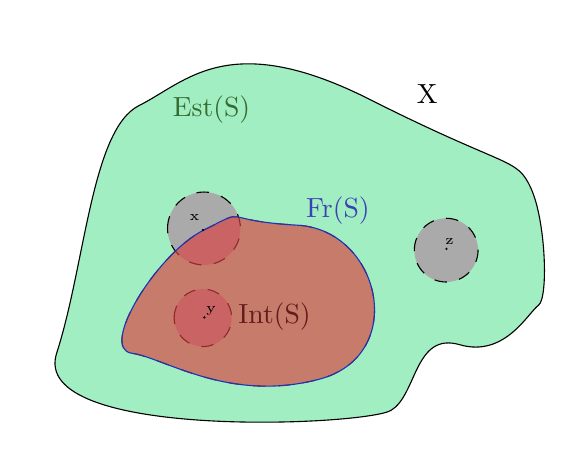
\begin{tikzpicture}[x=0.75pt,y=0.75pt,yscale=-1,xscale=1]
	%uncomment if require: \path (0,300); %set diagram left start at 0, and has height of 300
	
	%Shape: Polygon Curved [id:ds20780509926942758] 
	\draw  [fill={rgb, 255:red, 49; green, 219; blue, 119 }  ,fill opacity=0.46 ] (83.36,47.47) .. controls (106.2,36.05) and (126.53,10.19) .. (194.5,44.46) .. controls (262.46,78.73) and (265.28,72.05) .. (272.31,87.51) .. controls (279.33,102.96) and (280.73,140.19) .. (275.82,143.7) .. controls (270.9,147.21) and (259.66,168.99) .. (237.89,162.67) .. controls (216.11,156.34) and (217.34,186.75) .. (204.87,194.27) .. controls (192.41,201.8) and (30.01,208.95) .. (43.72,166.68) .. controls (57.42,124.42) and (60.51,58.89) .. (83.36,47.47) -- cycle ;
	%Shape: Ellipse [id:dp07267279293997198] 
	\draw  [fill={rgb, 255:red, 170; green, 170; blue, 170 }  ,fill opacity=1 ][dash pattern={on 4.5pt off 4.5pt}] (100.32,149.71) .. controls (100.32,142.06) and (106.53,135.85) .. (114.18,135.85) .. controls (121.83,135.85) and (128.04,142.06) .. (128.04,149.71) .. controls (128.04,157.36) and (121.83,163.57) .. (114.18,163.57) .. controls (106.53,163.57) and (100.32,157.36) .. (100.32,149.71) -- cycle ;
	%Shape: Circle [id:dp14301596472047673] 
	\draw  [fill={rgb, 255:red, 170; green, 170; blue, 170 }  ,fill opacity=1 ][dash pattern={on 4.5pt off 4.5pt}] (97.13,106.67) .. controls (97.13,96.98) and (104.99,89.11) .. (114.69,89.11) .. controls (124.39,89.11) and (132.25,96.98) .. (132.25,106.67) .. controls (132.25,116.37) and (124.39,124.23) .. (114.69,124.23) .. controls (104.99,124.23) and (97.13,116.37) .. (97.13,106.67) -- cycle ;
	%Shape: Polygon Curved [id:ds6715413886545399] 
	\draw  [color={rgb, 255:red, 165; green, 21; blue, 21 }  ,draw opacity=1 ][fill={rgb, 255:red, 219; green, 64; blue, 64 }  ,fill opacity=0.66 ][dash pattern={on 4.5pt off 4.5pt}] (114.69,107.38) .. controls (137.54,95.95) and (119.83,102.81) .. (159.81,105.09) .. controls (199.79,107.38) and (213.5,167.92) .. (170.09,179.34) .. controls (126.68,190.76) and (95.84,169.06) .. (79.85,166.77) .. controls (63.86,164.49) and (91.85,118.8) .. (114.69,107.38) -- cycle ;
	%Shape: Polygon Curved [id:ds9708889204352493] 
	\draw  [color={rgb, 255:red, 24; green, 55; blue, 182 }  ,draw opacity=1 ] (114.69,107.38) .. controls (137.54,95.95) and (119.83,102.81) .. (159.81,105.09) .. controls (199.79,107.38) and (213.5,167.92) .. (170.09,179.34) .. controls (126.68,190.76) and (95.84,169.06) .. (79.85,166.77) .. controls (63.86,164.49) and (91.85,118.8) .. (114.69,107.38) -- cycle ;
	%Shape: Ellipse [id:dp5122415642618744] 
	\draw  [fill={rgb, 255:red, 170; green, 170; blue, 170 }  ,fill opacity=1 ][dash pattern={on 4.5pt off 4.5pt}] (216.04,117.11) .. controls (216.04,108.63) and (222.91,101.76) .. (231.39,101.76) .. controls (239.87,101.76) and (246.74,108.63) .. (246.74,117.11) .. controls (246.74,125.59) and (239.87,132.46) .. (231.39,132.46) .. controls (222.91,132.46) and (216.04,125.59) .. (216.04,117.11) -- cycle ;
	%Flowchart: Connector [id:dp19505614998037069] 
	\draw  [fill={rgb, 255:red, 0; green, 0; blue, 0 }  ,fill opacity=1 ] (231.74,116.53) .. controls (231.74,116.41) and (231.64,116.31) .. (231.52,116.31) .. controls (231.39,116.31) and (231.29,116.41) .. (231.29,116.53) .. controls (231.29,116.66) and (231.39,116.76) .. (231.52,116.76) .. controls (231.64,116.76) and (231.74,116.66) .. (231.74,116.53) -- cycle ;
	%Flowchart: Connector [id:dp9853432682472757] 
	\draw  [fill={rgb, 255:red, 0; green, 0; blue, 0 }  ,fill opacity=1 ] (115.14,149.55) .. controls (115.14,149.42) and (115.04,149.32) .. (114.92,149.32) .. controls (114.79,149.32) and (114.69,149.42) .. (114.69,149.55) .. controls (114.69,149.67) and (114.79,149.77) .. (114.92,149.77) .. controls (115.04,149.77) and (115.14,149.67) .. (115.14,149.55) -- cycle ;
	%Flowchart: Connector [id:dp4161639041008799] 
	\draw  [fill={rgb, 255:red, 0; green, 0; blue, 0 }  ,fill opacity=1 ] (114.44,107.4) .. controls (114.44,107.28) and (114.34,107.18) .. (114.21,107.18) .. controls (114.09,107.18) and (113.99,107.28) .. (113.99,107.4) .. controls (113.99,107.53) and (114.09,107.63) .. (114.21,107.63) .. controls (114.34,107.63) and (114.44,107.53) .. (114.44,107.4) -- cycle ;
	
	% Text Node
	\draw (98.4,41.63) node [anchor=north west][inner sep=0.75pt]  [color={rgb, 255:red, 28; green, 85; blue, 24 }  ,opacity=1 ] [align=left] {\textcolor[rgb]{0.22,0.42,0.19}{Est(S)}};
	% Text Node
	\draw (130.03,141.01) node [anchor=north west][inner sep=0.75pt]   [align=left] {\textcolor[rgb]{0.39,0.11,0.11}{Int(S)}};
	% Text Node
	\draw (162.68,90.22) node [anchor=north west][inner sep=0.75pt]   [align=left] {\textcolor[rgb]{0.24,0.25,0.71}{Fr(S)}};
	% Text Node
	\draw (106.47,98.81) node [anchor=north west][inner sep=0.75pt]   [align=left] {{\tiny x}};
	% Text Node
	\draw (114.49,143.17) node [anchor=north west][inner sep=0.75pt]   [align=left] {{\tiny y}};
	% Text Node
	\draw (229.68,110.26) node [anchor=north west][inner sep=0.75pt]   [align=left] {{\tiny z}};
	% Text Node
	\draw (216,36) node [anchor=north west][inner sep=0.75pt]   [align=left] {X};
	
	
	\end{tikzpicture}
	
	\caption{In questo caso y è interno, x di frontiera e z esterno} \label{fig:Sottoinsiemi}
\end{figure}

\begin{osss} Con le notazioni precedenti valgono:
\begin{enumerate} 
	\item $ Int(S) \subset S $
	\item $Est(S) \subset \comp{X} S $
	\item $X=Int(S) \sqcup Est(S) \sqcup Fr(S) $
	\item $ S= Int(S) \sqcup ( S \cap Fr(S) ) $
	\item sono equivalenti le seguenti propietà : 
	\begin{itemize}
		\item $Fr(S) \subset S $
		\item $S = Int(S) \sqcup Fr(S) $ 
		\item $\comp{X} S \in \tau $, i.e. il complementare di S è aperto
	\end{itemize}
\end{enumerate}
\end{osss}

\begin{lem} L'interno di S è l'unione di tutti gli aperti contenuti in S, cioè il più grande aperto contenuto in S.
\end{lem}

\section{Chiusura}

\begin{deff}
Sia $(X, \tau )$ uno spazio topologico, un sottoinsieme C di X si dice chiuso in $\tau $ se il suo complementare è un aperto in $\tau $.
\end{deff}

\begin{oss} La famiglia dei chiusi di $\tau $ contiene l'insieme vuoto e l'insieme ambiente (X), è stabile per intersezione arbitraria e stabile per unione finita.
\end{oss}

\begin{lem} Se X è un insieme non vuoto e sia $\mathcal{F} \subset \Parts (X) $ tale che: $\mathcal{F} \ni \phi ,\, X$, sia stabile per intersezione arbitraria e stabile per unione finita; allora esiste un'unica topologia indotta $\tau $ su X che vede $\mathcal{F} $ come famiglia dei suo chiusi.
\end{lem}

\begin{deff}
Sia $(X, \tau )$ uno spazio topologico, dato un sottoinsieme S di X la chiusura di S è il più piccolo chiuso di $\tau $ contenente S, e si indica con $\bar{S} ^ {(X,\tau )} $ oppure $ Cl_{(X, \tau )} (S)$
\end{deff}

\begin{deff}
Sia $(X, \tau )$ uno spazio topologico, dato un sottoinsieme S di X. Un punto x di S si dice:
\begin{itemize}
	\item \emph{punto aderente} ad S in $(X, \tau )$ se ogni intorno di x ha intersezione non vuota con S.
	\item \emph{punto di accomulazione} di S in $(X, \tau )$ se per ogni intorno di x la sua intersezione con S contiene almeno un punto diverso da x stesso.
	\item \emph{punto isolato} di S in $(X, \tau )$ se è aderente ad S, ma non di accomulazione, o equivalentemente esiste un intorno U di x tale che $S \cap U = \{ x \} $.
\end{itemize}
inoltre si dice che:
\begin{itemize}
	\item L'insieme dei punti di accomulazione di S è detto il derivato di S in $(X, \tau )$ e lo indicheremo con $\mathcal{D}_{\tau } (S)$.
	\item L'insieme dei punti isolati di S lo indicheremo con $S^* $.
	\item L'insieme dei punti aderenti ad S è uguale a $ \mathcal{D}_{\tau } (S) \sqcup S^* $
\end{itemize}
\end{deff}	 

\begin{prop}
Sia $(X, \tau )$ uno spazio topologico, dato un sottoinsieme S di X allora x appartiene alla chiusura di S in $\tau $ se e solo se x è aderente ad S, ma quindi segue che: 
\begin{equation*}
\bar{S} ^{\tau} =   \mathcal{D}_{\tau } (S) \sqcup S^* 
\end{equation*}
\end{prop}

\begin{form}
Sia $(X, \tau )$ uno spazio topologico, dato un sottoinsieme S di X allora: 
\begin{enumerate}
	\item $ S \subset \bar{S} $
	\item $S$  è chiuso $\Leftrightarrow S = \bar{S} $
	\item $\mathcal{D} (S) = \bar{S} \backslash S^* $
	\item $\bar{S} = X \backslash Est(X) = Int(S) \sqcup Fr(S) = S \cup Fr(S) $
	\item $S \subset T \Rightarrow \bar{S} \subset \overline{T} $, i.e. l'operatore di chiusura è monotono
	\item$Fr(S) = \bar{S} \cap \overline{X \backslash S} $
\end{enumerate}
\end{form}

\section{Densità}

\begin{deff}
Sia $(X, \tau )$ uno spazio topologico, un sottoinsieme S di X si dice \emph{denso} se $X = \bar{S} $, inoltre sono equivalenti:
\begin{enumerate}
	\item S denso in $(X,\tau )$
	\item Dato un punto x di X, allora per ogni intorno U di x segue $U \cap S \neq \phi $
	\item Supponiamo che per ogni x in X sia assegnato un S.F.I. $\mathcal{V}_\tau (x) $ tale che per ogni $V \in \mathcal{V}_\tau (x)$ segua $V \cap S \neq \phi$ 
	\item $Int(X \backslash S ) = Est(S) = \phi $
	\item per ogni aperto A non vuoto segue che $A \cap S \neq \phi $
	\item esiste una base $\B$ per $\tau$ tale che $\forall B \in \B . \, B \cap S \neq \phi$
\end{enumerate}
\end{deff}

\section{Chiusura sequenziale}

\begin{deff} 
Sia $(X, \tau )$ uno spazio topologico, dato un sottoinsieme S di X definiamo la chiusura sequenziale di S in $(X,\tau)$ come:
\begin{equation*}
	\overline{S} ^{seq} := \{ x \in X | \exists \{x_n\} _{n\in \N } \subset S \text{ t.c. } \{x_n\} _{n\in \N } \to x \text{ in }(X,\tau) \}
\end{equation*}
\end{deff}

\begin{prop} 
Vale sempre che $ \overline{S} ^{seq} \subset \overline{S} $, nel caso in cui $(X,\tau)$ soddisfi il primo assioma di numerabilità allora vale l'eguaglianza ($ \overline{S} ^{seq} = \overline{S} $)
\end{prop}

\begin{ex}[Spazio topologico che non rispetta il primo assioma di nuberabilità e con chiusura sequenziale diversa da quella topologica]
Questo è $\R ^\R $ con  \emph{topologia della convergenza puntuale}. Per farlo definisco il sistema di intorni
\funmap{\mathcal{V} }{\R ^\R \times \Parts _F (\R ) \times \R ^+}{\Parts ( \Parts ( \R ^\R ) ) }{(f,I,\epsilon)}{\{g : \R \to \R : \, |g(t) - f(t)| < \epsilon, \, \forall t \in I \}}
e lo uso per indurre una topologia su $\R ^\R $, quest'ultima non soddisfa il primo assioma e se scelgo $S = \{ f:\R \to \R |\, f(i) = 0 \forall i \in \R $ tranne un numero finito di valori $\}$ avrò che $\bar{S} = \R ^\R$ ma $ (\equiv 1 ) \not \in \bar{S}^{seq}$.
\end{ex}

\begin{deff}
uno spazio topologico si dice separabile se ammette un sottoinsieme numerabile denso
\end{deff}

\begin{prop}
Uno spazio topologico a base numerabile è separabile
\end{prop}

\begin{oss}
Non vale il viceversa, basta definire su $\R$ la topologia indotta dalla base $\{ [a,b) | a,b \in \R , \, a < b \}$, la quale rispetta il primo assioma di numerabilità, lo spazio topologico è separabile, ma non ha base numerabile 
\end{oss}

\begin{prop}
	Se uno spazio topologico è metrizzabile e separabile allora è a base numerabile
\end{prop}

\section{Applicazioni tra spazi topologici}

\begin{deff}
Una applicazione tra spazi topologici $f:(X,\tau) \to (Y,\xi )$ si dice continua in $x \in X$ se per ogni intorno U di $f(x)$ per $\xi$ esiste un intorno V di x per $\tau$ tale che $f(V) \subset U $
\end{deff}

\begin{prop}
Data una applicazione tra spazi topologici $f:(X,\tau) \to (Y,\xi )$ sono equivalenti:
\begin{enumerate}
	\item $f$ continua in ogni punto di X (cioè $f$ continua)
	\item per ogni aperto di $\xi$ la sua controimmagine è un aperto di $\tau $, i.e. $\forall A \in \xi \to f\inv (A) \in \tau $
	\item per ogni chiuso di $\xi$ la sua controimmagine è un chiuso di $\tau $
\end{enumerate}


\tikzset{every picture/.style={line width=0.75pt}} %set default line width to 0.75pt        

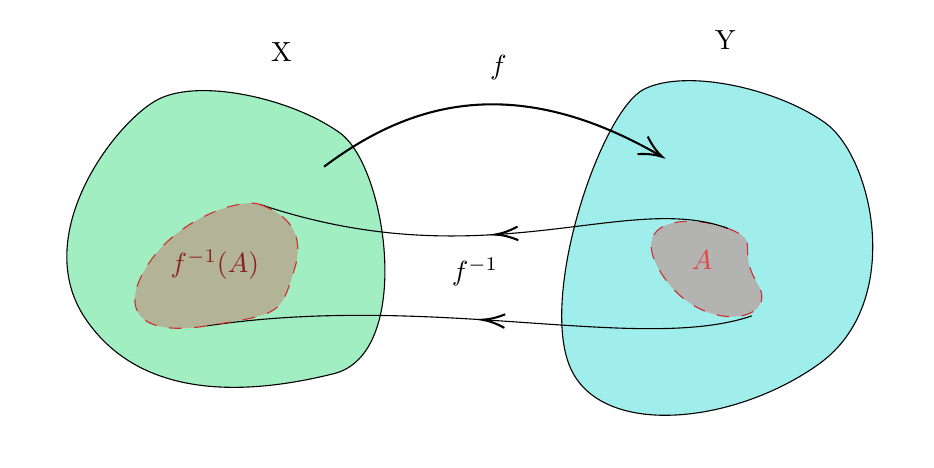
\begin{tikzpicture}[x=0.75pt,y=0.75pt,yscale=-1,xscale=1]
%uncomment if require: \path (0,300); %set diagram left start at 0, and has height of 300

%Shape: Polygon Curved [id:ds16526513362399742] 
\draw  [fill={rgb, 255:red, 49; green, 219; blue, 119 }  ,fill opacity=0.46 ] (192.48,42.45) .. controls (212.78,32.3) and (256.87,42.25) .. (279.8,58.75) .. controls (302.72,75.24) and (315.26,165.14) .. (276.92,174.72) .. controls (238.58,184.3) and (184.91,189.1) .. (157.26,148.36) .. controls (129.62,107.63) and (172.19,52.6) .. (192.48,42.45) -- cycle ;
%Shape: Polygon Curved [id:ds5254249579257063] 
\draw  [fill={rgb, 255:red, 49; green, 219; blue, 213 }  ,fill opacity=0.46 ] (426.35,37.66) .. controls (446.64,27.51) and (490.73,37.46) .. (513.66,53.95) .. controls (536.59,70.45) and (552,140.22) .. (510.78,169.93) .. controls (469.57,199.64) and (403.44,206.35) .. (390.02,169.93) .. controls (376.6,133.51) and (406.05,47.81) .. (426.35,37.66) -- cycle ;
%Curve Lines [id:da7424444324764179] 
\draw [line width=0.75]    (272.13,75.04) .. controls (310.28,46.43) and (360.76,27.31) .. (433.96,69.61) ;
\draw [shift={(435.07,70.25)}, rotate = 210.3] [color={rgb, 255:red, 0; green, 0; blue, 0 }  ][line width=0.75]    (10.93,-4.9) .. controls (6.95,-2.3) and (3.31,-0.67) .. (0,0) .. controls (3.31,0.67) and (6.95,2.3) .. (10.93,4.9)   ;
%Shape: Polygon Curved [id:ds40318824191580926] 
\draw  [color={rgb, 255:red, 206; green, 46; blue, 46 }  ,draw opacity=1 ][fill={rgb, 255:red, 207; green, 90; blue, 90 }  ,fill opacity=0.4 ][dash pattern={on 4.5pt off 4.5pt}] (466.7,104.75) .. controls (483.95,111.46) and (470.05,113.38) .. (481.07,131.59) .. controls (492.09,149.8) and (454.72,156.51) .. (435.55,127.76) .. controls (416.38,99) and (449.44,98.04) .. (466.7,104.75) -- cycle ;
%Curve Lines [id:da5510549835221298] 
\draw    (241.46,93.25) .. controls (349.76,129.67) and (417.81,86.54) .. (466.7,104.75) ;
\draw [shift={(354.64,107.72)}, rotate = 356.91] [color={rgb, 255:red, 0; green, 0; blue, 0 }  ][line width=0.75]    (10.93,-3.29) .. controls (6.95,-1.4) and (3.31,-0.3) .. (0,0) .. controls (3.31,0.3) and (6.95,1.4) .. (10.93,3.29)   ;
%Curve Lines [id:da5157101180402244] 
\draw    (215.58,151.72) .. controls (324.84,135.42) and (424.52,165.14) .. (478.2,146.92) ;
\draw [shift={(348.32,148.75)}, rotate = 3.46] [color={rgb, 255:red, 0; green, 0; blue, 0 }  ][line width=0.75]    (10.93,-3.29) .. controls (6.95,-1.4) and (3.31,-0.3) .. (0,0) .. controls (3.31,0.3) and (6.95,1.4) .. (10.93,3.29)   ;
%Shape: Polygon Curved [id:ds7519653574465133] 
\draw  [color={rgb, 255:red, 206; green, 46; blue, 46 }  ,draw opacity=1 ][fill={rgb, 255:red, 207; green, 90; blue, 90 }  ,fill opacity=0.4 ][dash pattern={on 4.5pt off 4.5pt}] (241.46,93.25) .. controls (250.08,96.61) and (264.46,103.79) .. (257.75,124.88) .. controls (251.04,145.97) and (252,145.97) .. (215.58,151.72) .. controls (179.16,157.47) and (173.89,141.05) .. (188.74,120.09) .. controls (203.6,99.12) and (232.83,89.9) .. (241.46,93.25) -- cycle ;

% Text Node
\draw (245.44,14.06) node [anchor=north west][inner sep=0.75pt]   [align=left] {X};
% Text Node
\draw (350.95,20.08) node [anchor=north west][inner sep=0.75pt]    {$f$};
% Text Node
\draw (459.18,8.31) node [anchor=north west][inner sep=0.75pt]   [align=left] {Y};
% Text Node
\draw (332.43,117.82) node [anchor=north west][inner sep=0.75pt]    {$f^{-1}$};
% Text Node
\draw (197,114) node [anchor=north west][inner sep=0.75pt]  [color={rgb, 255:red, 138; green, 32; blue, 32 }  ,opacity=1 ]  {$f^{-1}( A)$};
% Text Node
\draw (448,114) node [anchor=north west][inner sep=0.75pt]    {$\textcolor[rgb]{0.92,0.26,0.26}{A}$};


\end{tikzpicture}

\end{prop}

\begin{prop} La composizione di applicazioni continue è continua
\end{prop}

\begin{osss}
Data una applicazione tra spazi topologici $f:(X,\tau) \to (Y,\xi )$ qualsiasi:
\begin{itemize}
	\item l'applicazione costante è sempre continua
	\item la continuità si preserva per ogni $\tau ' \succ \tau$ su X e per ogni $\xi ' \prec \xi $ su Y
	\item se $\tau$ è la discreta allora $f$  è continua
	\item se $\xi $ è la banale allora $f$ è continua
\end{itemize}
\end{osss}

\begin{deff}
Data una applicazione tra spazi topologici $f:(X,\tau) \to (Y,\xi )$ diciamo che $f$ è aperta (chiusa) se manda aperti (chiusi) in aperti (chiusi)
\end{deff}

\begin{deff}
Data una applicazione tra spazi topologici $f:(X,\tau) \to (Y,\xi )$ si dice \emph{omemorfismo} se è bigettiva, continua e l'inversa è continua
\end{deff}

\begin{prop}
Data una applicazione tra spazi topologici $f:(X,\tau) \to (Y,\xi )$ sono equivalenti: 
\begin{enumerate} 
	\item f omemorfismo
	\item f è continua, bigettiva, aperta
	\item f è continua, bigettiva, chiusa
\end{enumerate}
\end{prop}

\begin{oss}
Se $f$ omemorfismo e definiamo $f(\tau) := \{ f(A) \in \Parts (Y) | \, A \in \tau \}$ allora $f(\tau ) = \xi$ e $f\inv (\xi ) = \tau $.
\end{oss}

\begin{prop} Sia $f:X \to Y $ un'applicazione tra insiemi non vuoti e sia $\xi $ una topologia su Y, allora $f\inv ( \xi) $ (detta immagine inversa di $\xi$ tramite f) è la topologia $\tau '$ meno fine su X tale che $f:(X,\tau') \to (Y,\xi )$ sia continua.
\end{prop}

\section{Sottospazi topologici}

\begin{deff} Sia $(X,\tau)$ spazio topologico e $S \subset X $ non vuoto, considero l'inclusione $i_S : S \xhookrightarrow{} X$, allora l'immagine inversa di $\tau $ tramite $i_S $ si dice topologia relativa su S indotta da $(X,\tau)$ e si indica con $\tau_S = \tau |_S := (i_S)\inv (\tau ) $ 
$(S,\tau_S) $ si dice sottospazio topologico di $(X,\tau)$.
\end{deff}

\begin{prop} 
Sia $(S,\tau_S) $ sottospazio topologico di $(X,\tau)$. Allora vale che:
\begin{enumerate}
	\item $\tau_S = \{ A\cap S | A \in \tau \}$
	\item Se F è chiuso su $\tau_S$ allora esiste un chiuso G di $\tau $ tale che $F=G\cap S $
	\item se $\	B $ è una base di $\tau $ allora $\B _S = \{B \cap S | B \in \B \} $ è una base di $\tau _S $ 
	\item se $\	mathcal(S) $ è una sottobase di $\tau $ allora $\mathcal(S) _S = \{B \cap S | B \in \mathcal(S) \} $ è una sottobase di $\tau _S $ 
	\item sia $x \in S$ allora $\mathcal{N}_{\tau_S} = \{ U \cap S | \, U \in \mathcal{N}_{\tau} \}$
	\item sia $x \in S$ e $\mathcal{V}_{\tau}$ un S.F.I. per x in $\tau$ allora $\mathcal{V}_{\tau_S} = \{ V \cap S | \, V \in \mathcal{V}_{\tau} \}$ per x in $\tau_S$
	\item sia $W \in \Parts (S) $ allora $\overline{W}^{\tau_S} =  \overline{W}^\tau \cap S$
	\item dati $T \subset S \subset X$ allora la topologia indotta da $(X,\tau)$ su T è la stessa indotta dalla topologia indotta da  $(X,\tau)$ su S su T. i.e. $(\tau |_S )|_T  =\tau |_T $
\end{enumerate}
\end{prop}

\begin{prop}
Data una applicazione tra spazi topologici continua $f:(X,\tau) \to (Y,\xi )$ valgono:
\begin{itemize}
 	\item $f|_S : (S, \tau|_S) \to (Y|\xi) $ è continua
	\item se $f(S) \subset T $ allora $f|_S^T : (S, \tau|_S) \to (Y, \xi|_T) $ è continua
\end{itemize}
\end{prop}

\begin{oss} in $(X,\tau)$, T,S non vuoti e tali che $T\subset S \subset X$ allora se S è aperto (chiuso) in $\tau$ e T aperto (chiuso) in $\tau_S$ allora T è aperto (chiuso) in $\tau$.
\end{oss}

\section{Prodotti topologici finiti}
In questa sezione abbrevieremo il prodotto coretesiano con la produttoria $\prod $.
\begin{prop}
	Sia $ n \in \Z ^+$ e dati $\{ X_i , \tau_i \}_{i=1}^n $ spazi topologici, allora l'insieme $\tau_1 \times ... \times \tau_n = \{ (A_1, ... , A_2) \in \Parts(X_1 \times ... \times X_n ) \, | \, \forall i \in {1,...,n} A_i \in \tau_i \}$ soddisfa: 
	\begin{itemize}
		\item  $\prod_{i=1}^{n} \tau_i $ è un ricoprimento di $\prod_{i=1}^n X_i$ .
		\item $siano A,B \in \prod_{i=1}^{n} \tau_i $ allora $A \cap B $ è unione di elementi di $\prod_{i=1}^{n} \tau_i $.
	\end{itemize}
Allora $\prod_{i=1}^{n} \tau_i $ è base di un'unica topologia $\tau$ (indicata anche con abuso di notazione $\left \langle \prod_{i=1}^{n} \tau_i  \right \rangle $), detta topologia prodotto di $\prod_{i=1}^{n} \tau_i $ su $\prod_{i=1}^{n} X_i $. Inoltre la coppia $(\prod_{i=1}^{n} X_i ,\tau )$ si dice spazio topologico prodotto (o prodotto topologico) di $\{ X_i , \tau_i \}_{i=1}^n $.
	
\end{prop}

\begin{prop}
	Nell'ambiente della precedente proposizione valgono le seguenti affermazioni:
	\begin{enumerate}
		\item Se $\beta _i $ base di $\tau_i$ per $i=1,...,n$ allora $\beta_1 \times ... \times \beta_n $ è base di $\tau $ 
		\item $\tau $ è la topologia meno fine che rende le proiezioni canoniche, cioè per ogni $i=1,...,n$ : 
			\funmap{p_i}{\prod_{j=1}^n X_j}{X_i}{(x_1,...,x_n)}{x_i}
		continue. 
		\item le proiezioni cononiche sono aperte per $\tau $, ma in generale non chiuse.
		\item sia $(x_i)_i \in \prod_{i=1}^n X_i $, sia $P \in \Parts (\prod_{i=1}^n X_i) $ allora: 
		\begin{equation*}
		P \in \mathcal{N}_\tau (x_1,...,x_n) \Leftrightarrow \forall i \, \exists U_i \in \mathcal{N}_{\tau_i} \, | \, U_1\times ... \times U_n \subset P 
		\end{equation*}
		\item se dato $x_i \in X_i $ è assegnato un S.F.I. $\mathcal{V}_i(x_i) $ di $x_i $ in $\tau_i$, per ogni $ i = 1,...,n $ allora segue che $\prod_{i=1}^n \mathcal{V}_i (x_i ) $ è un S.F.I. di $(\nesimo{x}{,}{n} ) $ in $\tau$.
		\item $f : (Y, \xi) \to ( \prod_{i=1}^n X_i , \tau ) $ con componenti $f = (f_i)_i $ allora :
		\begin{center}
			f continua in $\tau$ $\Leftrightarrow$ ogni componente $ f_i $ è continua in $\tau_i $
		\end{center}
		\item Sia $S_ i \in \Parts ( X_i ) $ per $i=1,...,n $ allora valgono : 
			\begin{equation*}
				\overline{ \left( \prod_{i=1}^{n} S_i \right) } ^\tau = \prod_{i=1}^{n}\overline{S_i}^{\tau_i} \text{ e } Int_\tau\left({\prod_{i=1}^{n} S_i} \right)  = \prod_{i=1}^{n}Int _{\tau_i} ({S_i} )
			\end{equation*}		
		\end{enumerate}
\end{prop}

\begin{osss}
	\begin{enumerate}
	\item Con questa costruzione potremmo avere problemi di corerenza infatti su $\R ^ n$ potremmo avere due topologie euclidee naturali:
	\begin{itemize}
		\item quella naturale indotta dalla base formata da tutte le palle aperte
		\item quella data dal prodotto topologico della retta euclidea $(\R ^n , \tau_e )$ con se stessa n volte
	\end{itemize}
	formunatamente si dimostra essere le stesse
	\item Potremmo avere un problema di \emph{coerenza filosofica} quando componiamo la restrizione di spazi topologici e il prodotto topologico, dati spazi topologici $(X_i,\tau_i) \, i=1,2$ e $S_1 \times S_2 \subset X_1 \times X_2$ sul sottoinsieme ho due topologie naturali :
	\begin{itemize}
		\item quella indotta dal prodotto topologico tra le due topologie ristrette 
		\begin{equation*}
			\left \langle \tau_1 |_{S_1} ,  \tau_2 |_{S_2} \right \rangle 
		\end{equation*}
		\item quella indotta dalla restrizione su quella indotto dal prodotto
		\begin{equation*}
			\left \langle \tau_1  ,  \tau_2  \right \rangle |_{S_1 \times S_2}
		\end{equation*}
	\end{itemize}
\end{enumerate}
\end{osss}

\begin{cor}
	Siano $(X_I,\tau_i) \: i=1,2$ spazi topologici e $(X_1 \times X_2 , \tau)$ spazio topologico prodotto allora per ogni $x_i \in X_i$ vale $\{x_1\}\times X_2$ è omemorfo a $X_2$ e $X_1 \times \{x_2\}$ è omemorfo a $X_1$
\end{cor}

\section{Topologia Quoziente}

\begin{deff}
	Sia $(X,\tau )$ spazio topologico e Y insieme non vuoto, $f : X \to Y $ applicazione. \\
	Allora la topologia quoziente su Y rispetto a f ( detta anche la topologia indotta da f su Y) è la top più fine su Y che rende continua f. La indicheremo con $\tau_f$.
\end{deff}

\begin{lem}
	Nelle ipotesi della definizione precedente valgono:
	\begin{enumerate}
		\item la topologia quoziente su Y rispetto a f esiste sempre ed è unica.
		\item 
		\[
			\tau_f := \left\{ A \in \Parts (Y) | f\inv (A) \in \tau \right\}
		\]
		\item Ha la seguente \textbf{propietà universale} (del quoziente topologico):\\
		supponiamo di dotare Y di $\tau _f $, allora per ogni apllicazione di spazi topologici $g:(Y,\tau_f ) \to (Z,\nu ) $ vale: 
		\[
		g \text{ continua } \Longleftrightarrow g\circ f \text{ continua }
		\]
		
	\end{enumerate}
\end{lem}

\begin{deff}
	sia $ f: X \to Y $ qualsiasi, e S un sottoinsieme di X, allora si dice che S è $f$-saturo se è unione delle su fibre:
	\[
		S = f\inv (f(S)) = \bigcup_{x\in S} f\inv (f(x))
	\]
\end{deff}

\begin{lem}
	Sia $(X,\tau )$ spazio topologico e Y insieme non vuoto, $f : X \to Y $ applicazione surgettiva. Dotiamo Y di topologia $\tau_f$, allora valgono\begin{enumerate}
		\item A è aperto di $\tau_f$ se e solo se esite un S aperto di $\tau$ f-saturo con $A=f(S)$, cioè:
		\[
			\tau_f = \{ A \in \Parts(Y) | \exists S \in \tau , \, f\inv (f(S)) = S, \, f(S) = A \}
		\]
		\item C è chiuso in $\tau_f$ se e solo se esiste un S chiuso di $\tau$ f-saturo con $C=f(S)$
	\end{enumerate}
\end{lem}

\begin{deff}
	Una applicazione tra spazi topologici $f: (X,\tau ) \to (Y,\xi ) $ si dice \textit{identificazione} se $\xi= \tau _f$. 
\end{deff}

\begin{prop}
	Data una applicazione tra spazi topologici $f: (X,\tau ) \to (Y,\xi ) $ continua e surgettiva, allora le seguenti condizioni sono equivalenti:
	\begin{enumerate}
		\item $ f $ è una identificazione
		\item $\forall A \in \Parts (Y) $ tale che $f\inv (A)\in \tau \Rightarrow A \in \xi $.
		\item Ogni aperto U di $\tau$ f-saturo la sua immagine $f(U) $ è un aperto di $\xi$.
		\item Ogni chiuso C di $\tau$ f-saturo la sua immagine $f(C) $ è un chiuso di $\xi$.
		
	\end{enumerate}
\end{prop}

\begin{ex}
		Un controesempio di funzione identificazione ne aperta ne chiusa è $\mathbb{1}_{[0,1)} : (\R,\tau_{\mathcal{E} })  \to (\{0,1\}, \tau_{\mathcal{B} }) $.
\end{ex}

\begin{lem}
	Una identificazione $f: (X,\tau ) \to (Y,\tau_f ) $ allora f è aperta (chiusa) se e solo se la f-saturazione ($f\inv(f(A))$) di ogni suo aperto (chiuso) è ancora un aperto (chiuso).
\end{lem}

\subsection{Relazioni di equivalenza su spazi topologici}
\begin{deff}
	Sia $(X,\tau)$ uno spazio topologico e sia \textit{R} una relazione di equivalenza su X, sia $\pi: X \to X/R$ la proiezione naturale al quoziente, allora la topologia su$X/R$ indotta da $\pi$ si duce \textit{topologia quoziente di $\tau$ modulo R} e la coppia $(X/R, \tau_{X/R})$ si dice \textit{spazio topologico quoziente} di $(X,\tau ) $ modulo R
\end{deff}

\begin{osss}
	consideriamo $\pi : (X,\tau) \to (X/R , \tau_{X/R})$, allora: 
	\begin{itemize}
		\item $\tau_{X/R}$ è la topologia più fine che rende continua $\pi$
		\item $\pi$ è una identificazione
		\item $\pi\inv (\pi (x)) = \{ y \in X | \pi(y) = \pi(x) \}= [x]_R $
		\item $A \in \Parts(X)$ è $\pi$-saturo se e solo se $A= \bigcup_{x \in A } [x]_R$ , cioè per ogni elemento x di A $[x]_R \subset A$ .
		\item Vale ovviamente che A è aperto di $\tau_{X/R}$ se esiste U aperto di $\tau$ $\pi$-saturo tale che $A=\pi (U)$.
	\end{itemize}
\end{osss}

\begin{lem}
	Sia $f : (X,\tau) \to (X',\tau')$ applicazione tra spazi topologici continua, siano R,R' relazioni di equivalenza su X,X' e $\pi$,$\pi'$ le proiezioni natuarali (come in figura):
	\[
	\begin{tikzcd}[column sep=large, row sep=large]
	X \ar[d, "\pi"'] \ar[r, "f"'] & X' \ar[d , "\pi'" ] \\
	X/R \ar[r, "f'"'] & X'/R'
	\end{tikzcd}
	\]
	Allora esiste un unica \textit{f'} che fa commutare il diagramma se e solo se $\forall x \in X$ vale $f([x]_R) \subset [f(x)]_{R'}$, cioè $\forall x,y \in X $ vale $xRy \Rightarrow f(x)R'f(y)$. Inoltre \textit{f'} è continua.
\end{lem}

\begin{teo}
\label{quoziente:omomorfismo}
	Sia $f : (X,\tau) \to (Y,\xi)$ una applicazione tra spazi topologici continua e surgettiva, allora possiamo definire una relazione di equivalenza: 
	\[
		x R_f y \Longleftrightarrow f(x) = f(y)
	\]
	per cui vale $ [x]_{R_f} = f\inv (f(x))$. Inoltre esiste un'unica g continua e biettiva tale che commuti il diagramma: 
	\[
	\begin{tikzcd}[column sep=large, row sep=large]
	X \ar[d, "\pi"'] \ar[r, "f"'] & Y  \\
	X/R_f \ar[ru, "g"'] 
	\end{tikzcd}
	\] 
	inoltre g è un omomorfismo se e solo se f è una identificazione.
\end{teo}

\begin{cor}
	Se $f : (X,\tau) \to (Y,\xi)$ è una identificazione allora $X/R_f \cong Y $
\end{cor}

\begin{cor}
	Sia $(X,\tau )$ spazio topologico e sia R una relazione di equivalenza su X, sia $\pi : X \to X/R $ la proiezione al quoziente. Dato $(X',\tau')$ spazio topologico e $f:X \to X' $ mappa continua e surgettiva tale che $\forall x \in X$ segue $f\inv (f(x)) = [x]_R $ (cioè $R=R_f$). Allora 
	\[ f \text{ identificazione } \Rightarrow X/R \cong X'\]
\end{cor}

\section{Spazi di Haussdorff}

\begin{deff}
	Sia $(X,\tau )$ uno spazio topologico, allora si dice $T_1$ se i singoletti sono chiusi, oppure equivalentemente se per ogni punto x di X l'intersezione di tutti gli intorni di x è \{x\}
\end{deff}
\begin{deff}
	Sia $(X,\tau )$ uno spazio topologico, allora si dice di Haussdorff, o $T_2$, se per ogni $x,y \in X$ se $x\neq y$ allora esistono U intorno di x e V intorno di y tale che $U \cap V \neq \phi $.
\end{deff}

\begin{oss}
	Essere $ T_2 $ (o $T_1$) è una propietà topologica, cioè se esiste un omeomorfismo tra X e Y spazi topologici allora: 
	\begin{center}
		X è $T_2$ $\Longleftrightarrow $ Y è $T_2$
	\end{center}
\end{oss}

\begin{prop}
	Se $(X,\tau)$ è spazio topologico $T_2$ allora è anche $T_1$ 
\end{prop}

\begin{prop}
	Se $(X,\tau )$ uno spazio topologico $T_2$ e $S\subseteq X$ allora lo spazio topologico indotto su S è $T_2$
\end{prop}

\begin{prop}
	Siano $(X_I,\tau_i) \: i=1,2$ spazi topologici e $(X_1 \times X_2 , \tau)$ spazio topologico prodotto allora:
	\begin{center}
		$X_1, \, X_2$ sono $T_2$ $ \Longleftrightarrow $ $X_1\times X_2$ è $T_2$
	\end{center}
\end{prop}

\begin{prop}
	In uno spazio topologico di Haussdorff una serie convergente, allora converge ad un unico valore
\end{prop}

\begin{prop}
	\xtausptop, allora X è di Haussdorff se e solo se $\Delta_X = \{ (x,x) \in X \times X \,|\, x \in X \}$ è un chiuso della topologia prodotto di X con se stesso
\end{prop}
\section{Compattezza}

\begin{deff}
	Uno spazio topologico si dice compatto se da ogni ricoprimento aperto è possibile estrarre un sottoricoprimento finito
\end{deff}

\begin{deff}
	Dato uno spazio topologico $(X,\tau)$ e S sottoinsieme di X non vuoto, allora S si dice \textit{sottoinsieme compatto} di $(X,\tau)$ se lo è il sottospazio topologico indotto $(S,\tau |_S)$
\end{deff}

\begin{oss}
	Nelle ipotesi precedenti S è (sottoinsieme) compatto se e solo se per ogni famiglia di aperti che ricoprono S in X posso estrarne un sottofamiglia finita che lo ricopre ancora, i.e.
	\[
	\forall \{A_i\}_{i\in I} \subset \tau \text{ t.c. } \bigcup_{i \in I } A_i \supset S \text{ allora } \exists J \subset I \text{ finito, t.c. }  \bigcup_{i \in J } A_i \supset S   \]
\end{oss}

\begin{teo} [di Heine-Borel] 
	Ogni intervallo chiuso e limitato di $(\R , \tau_{\mathcal{E} })$, cioè della forma $[a,b]$, è un compatto
\end{teo}

\begin{oss}
	Non è sempre vero che un sottoinsieme di un compatto è un compatto: ad esempio $(0,1]$ non è compatto in $([0,1],\tau_{\mathcal{E} }|_S)$
	
\end{oss}

\begin{prop}
	\begin{enumerate}
		\item un sottoinsieme chiuso in uno spazio topologico compatto è compatto
		\item In uno spazio topologico $T_2$ ogni sottoinsieme compatto è chiuso
	\end{enumerate}
\end{prop}

\begin{cor}
	Sia $(\R , \tau_{\mathcal{E} })$ la retta reale con topologia euclidea, dato un sottoinsieme S non vuoto, allora S è compatto se e solo se è chiuso e limitato
\end{cor}

\begin{prop}
	Sia $(X,\tau)$ spazio topologico compatto e $(Y,\xi)$ uno spazio topologico qualsiasi. Data una applicazione continua di spazi topologici $f:X\to Y$. Allora $f(X)$ è compatto.
\end{prop}

\begin{cor} [Weiestrass]
	Sia $(X,\tau)$ uno spazio topologico compatto e $f:(X,\tau) \to (\R , \tau_{\mathcal{E} })$ allora esistono in X un punto di minimo e uno di massimo (non necessariamente unici).
\end{cor}

\begin{teo} [di Tychonoff]
	Data una famiglia finita di spazi topologici $\{ (X_i , \tau_i)\}_{i=1}^n$ allora $\prod_{i=1}^n X_i$ con la topologia prodotto è compatto se e solo se lo è $(X_i , \tau_i)$ per ogni i tra 1 e n
	
\end{teo}

\begin{cor} [quasi vero teorema di Heinde Borel]
	Un sottoinsieme non vuoto di $(\R^n ,\tau_{\mathcal{E} })$ è compatto se e solo se è chiuso e limitato
	
\end{cor}

\begin{prop}

	Data una applicazione di spazi topologici continua, se il dominio è compatto e il codominio è uno spazio di Haussdorff allora l'applicazione è chiusa. \\
	In particolare se l'applicazione è anche bigettiva è un omemorfismo.
\end{prop}

\begin{cor}
	Al teorema \ref{quoziente:omomorfismo} possiamo aggiungere che se $(X,\tau)$ è uno spazio compatto e $(Y,\xi)$ è uno spazio di Haussdorff allora g è un omemorfismo e f una identificazione
\end{cor}

\section{Connessione}

\begin{deff}
	Uno spazio topologico $(X,\tau )$ si dice connesso se non esistono sottoinsiemi di X non vuoti, proprio sia aperti che chiusi. \\
	Uno spazio si dice sconnesso se non è connesso.\\
	Un sottoinsieme S di X dice connesso (sconnesso) se lo è lo spazio topologico $(S, \tau |_S )$
	
\end{deff}

\begin{prop}
	Dato $(X, \tau)$ spazio topologico, le seguenti condizioni sono equivalenti:
	\begin{enumerate}
		\item X è sconnesso
		\item X si può esprimere come unione disgiunta di due aperti non vuoti
		\item X si può esprimere come unione disgiunta di due chiusi non vuoti
	\end{enumerate}
\end{prop}

\begin{deff}
	Un sottoinsieme S di $\R ^n$ si dice \textit{convesso} se per ogni x,y $\in S $ il segmento [x,y] è contenuto in S
\end{deff}

\begin{teo}
	Un sottoinsieme non vuoto di $\R$ è un intervallo (quindi convesso) se e solo se è un connesso
\end{teo}

\begin{oss}
	La connessione è una propietà topologica
\end{oss}

\begin{prop}
	Sia $f : (X , \tau) \to (Y,\tau) $ una applicazione continua tra spazi topologici e sia C un sottoinsieme connesso di X, allora f(C) è un sottoinsieme connesso di Y.
\end{prop}

\begin{oss}
	Sia $ (X,\tau) $ uno spazio topologico connesso e R una relazione di equivalenza su X, allora lo spazio topologico $(X/R , \tau |_{X/R})$ 
\end{oss}

\begin{deff}
	Sia $(X, \tau )$ spazio topologico e siano x,y punti di X, allora si dice che x,y sono connessi in $(X,\tau)$ se esiste un sottoinsieme connesso S di X tale che x,y sono contenuti in S
\end{deff}

\begin{lem}
	\xtausptop , possiamo definire la relazione di connessione come : 
	\begin{center}
		$x \rho y $ $\Longleftrightarrow $ x,y sono connessi in $(X,\tau)$
	\end{center}
	Allora $\rho$ è una relazione di equivalenza.\\
	Inoltre le $\rho$-classi di equivalenza si dicono componenti connsesse di $(X,\tau)$ 
\end{lem}

\begin{prop}
	\xtausptop, siano A,B sottoinsiemi connessi di $(X,\tau)$ con intersezione non nulla, allora $A \cup B $ è connesso
\end{prop}

\begin{prop}
	\xtausptop, allora X è connsesso $\Longleftrightarrow$ per ogni coppia di punti x,y $\in X$: x è connesso a y
\end{prop}

\begin{lem}
	\xtausptop e siano Y,Z sottoinsiemi di X tali che $ Y \subset Z \subset \overline{Y}$ allora Y connesso implica Z connesso

\end{lem}

\begin{cor}
	Banalmente segue che Y connesso implica $\overline{Y}$ connesso
\end{cor}

\section{Connessione per archi}

\begin{deff}
	\xtausptop, si dice connsesso per archi se per ogni coppia di punti x,y di X esiste un arco che li conginuge: cioè una funzione continua $ \alpha : [0,1] \to X $ tale che $\alpha (0)=x$ e $\alpha (1)=y$.
	Un sottoinsieme S di X è connesso per archi se lo è come sottospazio topologico
\end{deff}
	
\begin{oss}
	Ovviamente uno spazio topologico connesso per archi è connesso, ma non è vero il viceversa: un controesempio semplice è la chiusura del grafico di $\sin (x\inv )$
\end{oss} 

\begin{lem}
	Se X è connesso e localmente euclideo allora è connesso per archi
\end{lem}

\end{document}